\documentclass{article}

% Macros to make this problem look like the rest of our problems.
\usepackage{icpc_problem}

\usepackage{graphicx}

% Title of your problem.
\title{E: Coconut Calamity}

% Who made the problem
\author{Sean Egan}

% Keywords, from a set of standard keywords.
\keywords{problem}

% Anything you want to say about the problem, including how one could solve it
\comments{comment}

% Difficulty on a 1..10 scale.
\difficulty{1}

\begin{document}

% Plain English description of the problem
\begin{problemDescription}
Honeycomb Havoc is a mini-game from Mario Party 2, where you and your friends are trying to catch some fruits, and strangely coins, from a tree. Each player gets to take some items from the tree, then move to the back of the line to wait their turn again. The number of items you catch doesn't really matter, as long as none of them are the dreaded honeycomb. Catching the honeycomb causes the bees to swarm and attack you, which is totally not a good time.

\begin{center}
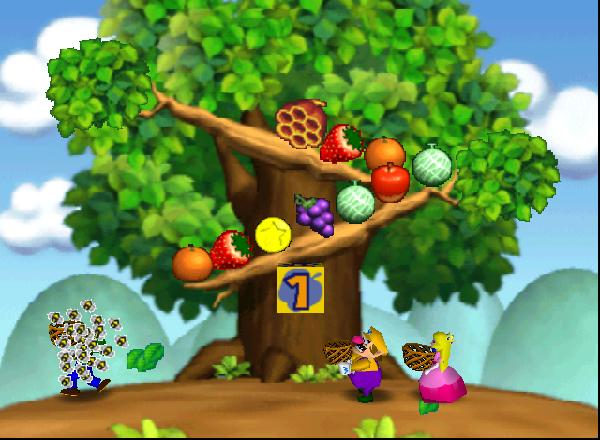
\includegraphics[height=7.5cm]{images/honeycomb-havoc.jpg}
\\
\caption{The original Honeycomb Havoc game}
\label{fig:sp500_long_results_zoomed}
\end{center}

In the classic Honeycomb Havoc game, you are allowed to choose between taking either one or two items. In our variant of the game, Coconut Calamity, you must take at least one item from the tree, with a maximum of $K$ items that can be taken in a single turn.

The tree in Coconut Calamity consists of some number of fruits, followed by a series of coconuts. Taking fruits is totally safe, but if you take even just one coconut, they were all topple over on your head, eliminating you from the game and giving you a serious headache.

After some number of turns, all but one of your friends have gotten hit on the head with a coconut. You're entering the final round, and this time it's for all the marbles. There are exactly $N$ fruits remaining in the tree, followed by several coconuts.

It's your turn to take items from the tree. Given that your friend has learned the best strategy possible for any game of Coconut Calamity, and they will always make the best move possible, you must determine whether it is possible for you to win the game or not.

\end{problemDescription}

% Specific input definition
% Includes what is being taken as input, and in what format
\begin{inputDescription}
The first line contains only an integer $0 \leq t \leq 10^5$, representing the number of games to play. The following $t$ lines contain two integers, $0 \leq N \leq 10^5$ and $1 \leq K \leq 10^5$, separated by a space.

As mentioned before, the integer $N$ represents the number of fruits remaining before the coconuts are being taken from the tree, and the integer $K$ is the maximum number of items that can be taken from the tree in any one turn.

\end{inputDescription}

% Specific output definition
% Includes what should be printed, and in what format
\begin{outputDescription}
If you can win the game, output "Winner", or if you're guaranteed to lose the game, output "Loser". Each game's output should be on its own line.

\end{outputDescription}

\begin{sampleInput}

3
2 2
3 2
3 5
\end{sampleInput}
\begin{sampleOutput}

Winner
Loser
Winner
\end{sampleOutput}

\end{document}